%% Template.tex; Solar Physics
%% 
\documentclass[namedreferences]{SolarPhysics}
%
% spr-sola-addons available options:
%  natbib        -- For citations: redefine \cite commands
%  solaenum      -- makes enumerated list with italics-roman numerals and a single right-bracket
%  linksfromyear -- loads a natbib and puts a link on a year citation (hyperref must be loaded)
%  optionalrh    -- for optional running title/author
%
\usepackage[optionalrh,solaenum]{spr-sola-addons} % For Solar Physics 
%\usepackage{epsfig}                     % For eps figures, old commands
\usepackage{graphicx}                    % For eps figures, newer & more powerfull
%\usepackage{courier}                    % Change the \texttt command to courier style
%\usepackage{amssymb}                    % useful mathematical symbols
\usepackage{color}                       % For color text: \color command
\usepackage{url}                         % For breaking URLs easily trough lines
\def\UrlFont{\sf}                        % define the fonts for the URLs


%% Local definitions
%% please place your own definitions here and don't use \def but
%% \newcommand{}{} or 
%% \renewcommand{}{} if it is already defined in LaTeX



%%%%%%%%%%%%%%%%%%%%%%%%%%%%%%%%%%%%%%%%%%%%%%%%%%%%%%%%%%%%%%%%%%
\begin{document}

\begin{article}

\begin{opening}

\title{THE HELIO 100 CME CHALLENGE}

%%%%%%%%%%%%%%%%%%%%%%%%%%%%%%%%%%%%%%%%%%%%%%%%%%%
%% Authors Names
%
\author{I.~\surname{}%$^{1}$\sep
%        I.~\surname{}$^{1}$\sep
%        I.~\surname{}$^{2}$      
       }

%%%%%%%%%%%%%%%%%%%%%%%%%%%%%%%%%%%%%%%%%%%%%%%%%%%
%% Runningheads
%
%\runningauthor{}
%\runningtitle{}


%%%%%%%%%%%%%%%%%%%%%%%%%%%%%%%%%%%%%%%%%%%%%%%%%%%
%% Affilations 
%
  \institute{$^{1}$ First affiliation
                     email: \url{e.mail-a} email: \url{e.mail-b}%\\ 
%             $^{2}$ Second affiliation
%                     email: \url{e.mail-c} \\
             }


%%%%%%%%%%%%%%%%%%%%%%%%%%%%%%%%%%%%%%%%%%%%%%%%%%%
%%% Abstract 
\begin{abstract}

Studying the impact of solar events throughout the heliosphere is of great importance for understanding and predicting space weather conditions. The Heliophysics Integrated Observatory (HELIO) was generated out of a need to link the detections of solar-driven events throughout the heliosphere, as they are detected via remote-sensing and in-situ instruments onboard various spacecrafts throughout our solar system.  Having been under development since 2009, HELIO is now at a stage of great scientific benefit for large scale studies, through the generation of workflows that use HELIO to access and cross-correlate lists of different solar events and their various measured properties.

%Geomagnetic storms at Earth can cause adverse effects on global communication networks, satellite operations, and human space travel. This is of increased importance in the current era of complex global communication systems, space-based communication systems, human space travel, and especially their potentially adverse effects in the vicinity of the Earth.


The fourth HELIO coordinated data analysis workshop (HELIO CDAW-4) held in Trinity College Dublin in September 2012 described three challenges to be addressed by focused working groups, comprising solar physicists and computer scientists alike. In this paper we outline the success of Challenge 2: ``The 100 CME Challenge". This challenge focused on using HELIO to study the origin, propagation and impacts of a large number of coronal mass ejections (CMEs) in the Heliosphere. HELIO provides an interface that allows researchers to track active regions as they evolve and produce solar flares and CMEs. Once launched, CMEs can be tracked in coronagraph and heliospheric images. Their impacts throughout the Heliosphere can then be measured using in-situ instruments from a number of spacecraft throughout the Heliosphere. The aim of this challenge is to use HELIO to track a large number of CMEs that had an associated type II radio burst from their source region, and possible flare occurrence, from the surface of the Sun to their effects through interplanetary space and at the planets. This was achieved through the generation of a workflow that accessed the corresponding event lists and used a ballistic CME model to predict its arrival time at Earth and elsewhere in the solar system. Thus providing a timeframe for determining the in-situ parameters measured at the different spacecraft locations where the CME impact occurred.

\end{abstract}



%%%%%%%%%%%%%%%%%%%%%%%%%%%%%%%%%%%%%%%%%%%%%%%%%%%
%% Keywords
%
%\keywords{}


\end{opening}
%-------------------------------------------------

%%%%%%%%%%%%%%%%%%%%%%%%%%%%%%%%%%%%%%%%%%%%%%%%%%%
%% Sections
%
% \section{}%\label{s:?} 
\section{Introduction}

\begin{figure} 
\centerline{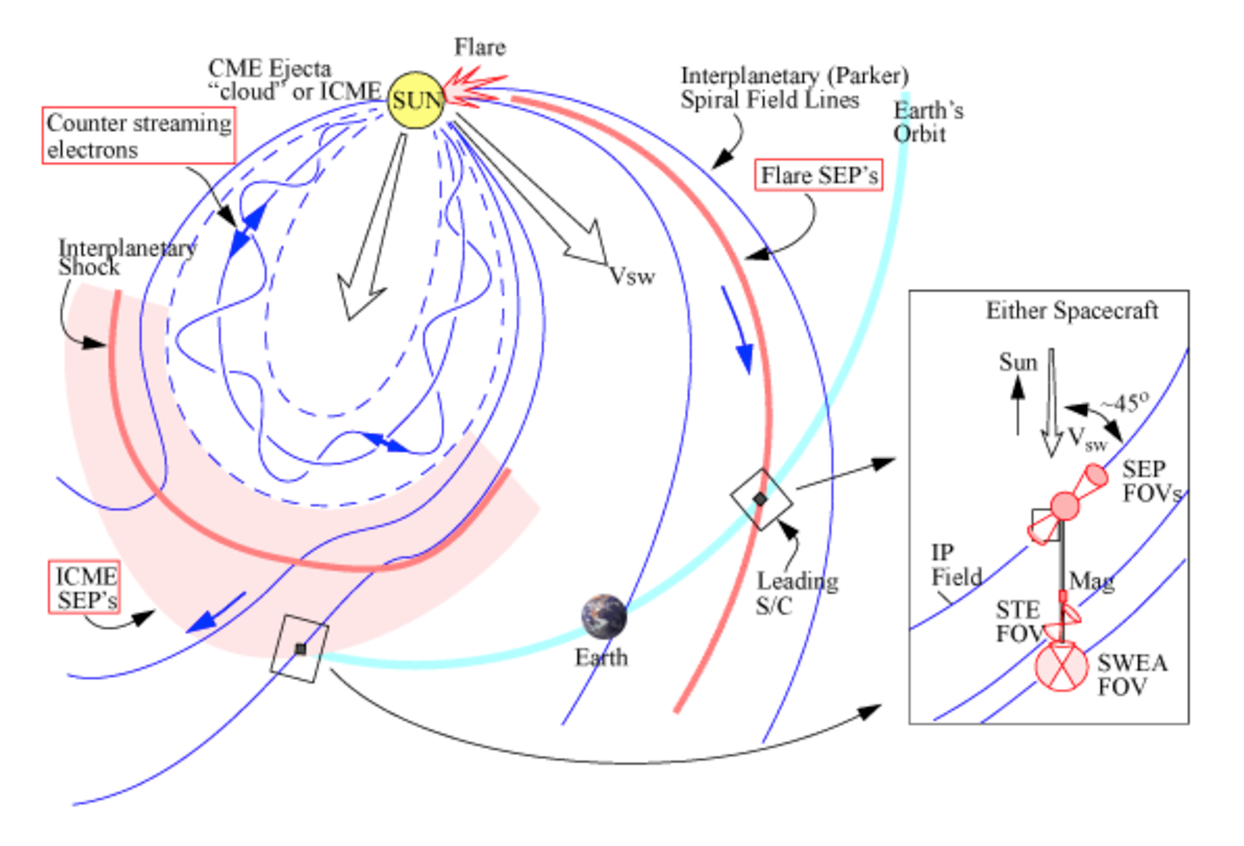
\includegraphics[width=\textwidth, clip=]{images/science_of_impact_c.pdf}}
\caption{}%\label{fig:?}
\end{figure}

\section{Building a workflow}

The challenge group began by choosing a `test case' CME for tracking through the HELIO interface, and building a model workflow to be ultimately extended for a large scale study of multiple events. The CME chosen was a fast event associated with a flare and type II radio burst, as listed in the ``Wind/WAVES type II bursts and CMEs" list \footnote{http://cdaw.gsfc.nasa.gov/CME\_list/radio/waves\_type2.html}. The radio burst was detected at 04:20~UT on 11~April~2004, with an associated NOAA C\,9.6 flare at disk location S\,14\,W\,47, and CME observed  in LASCO at 04:30~UT with central position angle 203$^{\circ}$, angular width 314$^{\circ}$, and speed 1645\,km\,s$^{-1}$.

The workflow was built in the following manner:






%% Figure 
%
% \begin{figure} 
% \centerline{\includegraphics[width=0.5\textwidth,clip=]{<fig.eps>}}
% \caption{}%\label{fig:?}
% \end{figure}



%% Table
%
% \begin{table}
% \caption{}%\label{tbl:?}
% \begin{tabular}{}     
% \hline
% \multicolumn{2}{c}{<>}
% <data>
% \hline
% \end{tabular}
% \end{table}
  

%%%%%%%%%%%%%%%%%%%%%%%%%%%%%%%%%%%%%%%%%%%%%%%%%%%%%%%%%%%%%%%%%%%%%%%%%%%
%% Appendix
%
% \appendix   



%%%%%%%%%%%%%%%%%%%%%%%%%%%%%%%%%%%%%%%%%%%%%%%%%%%%%%%%%%%%%%%%%%%%%%%%%%%
%% Acknowledgements
%
% \begin{acks}
%
% \end{acks}


%%% %%%%%%%%%%%%%%%%%%%%%%%%%%%%%%%%%%%%%%%%%%%%%%%%%%%%%%%%%%%
%% Bibliography
%
% Using BibTeX
%
%\bibliographystyle{spr-mp-sola}
\bibliographystyle{spr-mp-sola-cnd} %% Alternative style: no title, no concluding page
\bibliography{references.bib}  
%
% Without BibTeX 
% \begin{thebibliography}{}
% \bibitem[\protect\citeauthoryear{Author}{Year}]{key}
%   <bibliographical entry>
%
% \bibitem[\protect\citeauthoryear{}{}]{}
%   
%  
% \end{thebibliography}

\end{article} 
\end{document}
